%% LyX 2.2.2 created this file.  For more info, see http://www.lyx.org/.
%% Do not edit unless you really know what you are doing.
\documentclass[spanish]{article}
\usepackage[T1]{fontenc}
\usepackage[latin9]{inputenc}
\usepackage{geometry}
\geometry{verbose,tmargin=2cm,bmargin=2cm,lmargin=2cm,rmargin=2cm}
\usepackage{array}
\usepackage{float}
\usepackage{booktabs}
\usepackage{multirow}
\usepackage{graphicx}

\makeatletter

%%%%%%%%%%%%%%%%%%%%%%%%%%%%%% LyX specific LaTeX commands.
%% Because html converters don't know tabularnewline
\providecommand{\tabularnewline}{\\}

\makeatother

\usepackage{babel}
\addto\shorthandsspanish{\spanishdeactivate{~<>}}

\begin{document}

\section{Ejercicio 1}

\subsection{Implementacion Maquina de Moore}

\begin{figure}[H]
\begin{centering}
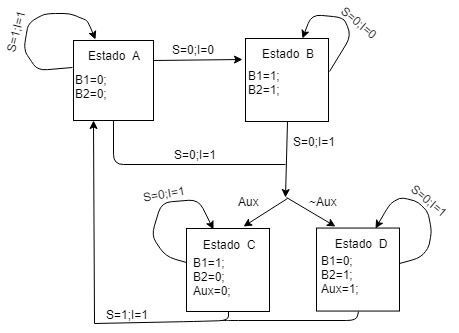
\includegraphics[scale=0.7]{Ej1_Moore_Diagrama}
\par\end{centering}
\caption{Diagrama Bloque}
\end{figure}
\begin{figure}[H]
\begin{centering}
\begin{tabular}{cccccccc}
\toprule 
\multirow{3}{*}{\textbf{Present State}} & \multicolumn{4}{c}{\textbf{Next State}} & \multirow{4}{*}{\textbf{B1}} & \multirow{4}{*}{\textbf{B2}} & \multirow{4}{*}{\textbf{Aux}}\tabularnewline
\cmidrule{2-5} 
 & \multirow{2}{*}{\textbf{S=1 I=1}} & \multirow{2}{*}{\textbf{S=0 I=0}} & \multicolumn{2}{c}{\textbf{S=0 I=1}} &  &  & \tabularnewline
\cmidrule{4-5} 
 &  &  & \textbf{Aux} & \textbf{\textasciitilde{}Aux} &  &  & \tabularnewline
\cmidrule{1-5} 
$y_{2}y_{1}$ & $Y_{2}Y_{1}$ & $Y_{2}Y_{1}$ & $Y_{2}Y_{1}$ & $Y_{2}Y_{1}$ &  &  & \tabularnewline
\midrule 
$A=00$ & $00$ & $01$ & $10$ & $11$ & $0$ & $0$ & $Aux(t-1)$\tabularnewline
\midrule 
$B=01$ & $00*$ & $01$ & $10$ & $11$ & $1$ & $1$ & $Aux(t-1)$\tabularnewline
\midrule 
$C=10$ & $00$ & $01$ & $10$ & $10$ & $1$ & $0$ & $0$\tabularnewline
\midrule 
$D=11$ & $00$ & $01$ & $11$ & $11$ & $0$ & $1$ & $1$\tabularnewline
\bottomrule
\end{tabular}
\par\end{centering}
\caption{Tabla de Estados}
\end{figure}
\begin{figure}[H]
\centering{}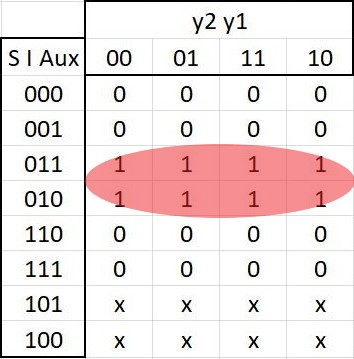
\includegraphics[scale=0.5]{Ej1_Moore_KY2.jpeg}\caption{Mapa Karnaugh $Y_{2}$}
\end{figure}

\[
Y_{2}=\overline{S}I
\]

\begin{figure}[H]
\begin{centering}
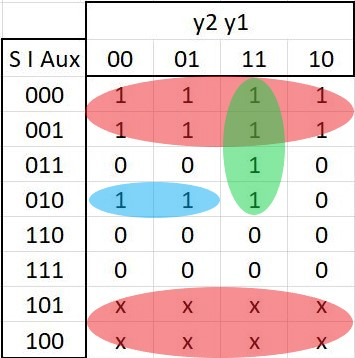
\includegraphics[scale=0.5]{Ej1_Moore_KY1.jpeg}
\par\end{centering}
\centering{}\caption{Mapa Karnaugh $Y_{1}$}
\end{figure}

\[
Y_{1}=\bar{I}+\bar{S}y_{2}y_{1}+\bar{Aux}\bar{S}\bar{y_{2}I}
\]

\begin{figure}[H]
\begin{centering}
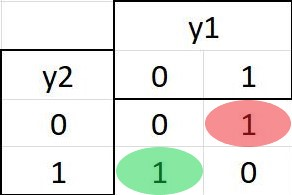
\includegraphics[scale=0.5]{Ej1_Moore_KB1.jpeg}
\par\end{centering}
\centering{}\caption{Mapa Karnaugh $B_{1}$}
\end{figure}

\[
B_{1}=y_{1}\oplus y_{2}
\]

\begin{figure}[H]
\begin{centering}
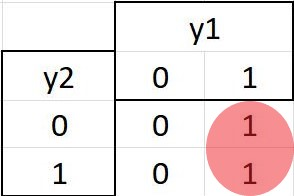
\includegraphics[scale=0.5]{Ej1_Moore_KB2.jpeg}
\par\end{centering}
\centering{}\caption{Mapa Karnaugh $B_{2}$}
\end{figure}

\[
B_{2}=y_{1}
\]


\subsection{Implementacion Maquina de Mealy}

\begin{figure}[H]
\begin{centering}
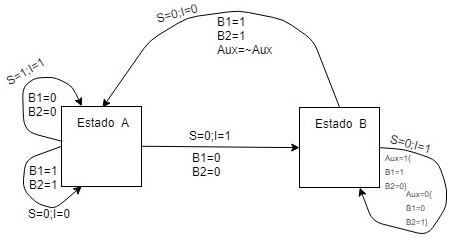
\includegraphics[scale=0.7]{Ej1_Mealy_Diagrama}
\par\end{centering}
\caption{Diagrama Bloque}
\end{figure}
\begin{figure}[H]
\begin{raggedright}
\begin{tabular}{cccccccccccccccc}
\toprule 
\textbf{\tiny{}Present State} & \multicolumn{3}{c}{\textbf{\tiny{}Next State}} & \multicolumn{12}{c}{\textbf{\tiny{}Out}}\tabularnewline
\midrule
\midrule 
\multirow{3}{*}{\textbf{\tiny{}y}} & \textbf{\tiny{}S=1 I=1} & \textbf{\tiny{}S=0 I=0} & \textbf{\tiny{}S=0 I=1} & \multicolumn{3}{c}{\textbf{\tiny{}S=1 I=1}} & \multicolumn{3}{c}{\textbf{\tiny{}S=0 I=0}} & \multicolumn{6}{c}{\textbf{\tiny{}S=0 I=1}}\tabularnewline
\cmidrule{2-16} 
 & \multirow{2}{*}{\textbf{\tiny{}Y}} & \multirow{2}{*}{\textbf{\tiny{}Y}} & \multirow{2}{*}{\textbf{\tiny{}Y}} & \multirow{2}{*}{\textbf{\tiny{}B1}} & \multirow{2}{*}{\textbf{\tiny{}B2}} & \multirow{2}{*}{\textbf{\tiny{}Aux}} & \multirow{2}{*}{\textbf{\tiny{}B1}} & \multirow{2}{*}{\textbf{\tiny{}B2}} & \multirow{2}{*}{\textbf{\tiny{}Aux}} & \multicolumn{3}{c}{\textbf{\tiny{}Aux=1}} & \multicolumn{3}{c}{\textbf{\tiny{}Aux=0}}\tabularnewline
\cmidrule{11-16} 
 &  &  &  &  &  &  &  &  &  & \textbf{\tiny{}B1} & \textbf{\tiny{}B2} & \textbf{\tiny{}Aux} & \textbf{\tiny{}B1} & \textbf{\tiny{}B2} & \textbf{\tiny{}Aux}\tabularnewline
\midrule 
{\tiny{}$A=0$} & {\tiny{}$0$} & {\tiny{}$0$} & {\tiny{}$1$} & {\tiny{}$0$} & {\tiny{}$0$} & {\tiny{}$Aux(t-1)$} & {\tiny{}$1$} & {\tiny{}$1$} & {\tiny{}$Aux(t-1)$} & {\tiny{}$0$} & {\tiny{}$0$} & {\tiny{}$Aux(t-1)$} & {\tiny{}$0$} & {\tiny{}$0$} & {\tiny{}$Aux(t-1)$}\tabularnewline
\midrule 
{\tiny{}$B=1$} & {\tiny{}$0$} & {\tiny{}$0$} & {\tiny{}$1$} & {\tiny{}$0$} & {\tiny{}$0$} & {\tiny{}$\bar{Aux(t-1)}$} & {\tiny{}$1$} & {\tiny{}$1$} & {\tiny{}$\bar{Aux(t-1)}$} & {\tiny{}$1$} & {\tiny{}$0$} & {\tiny{}$Aux(t-1)$} & {\tiny{}$0$} & {\tiny{}$1$} & {\tiny{}$Aux(t-1)$}\tabularnewline
\bottomrule
\end{tabular}
\par\end{raggedright}
\caption{Tabla de Estados}
\end{figure}

\begin{figure}
\begin{centering}
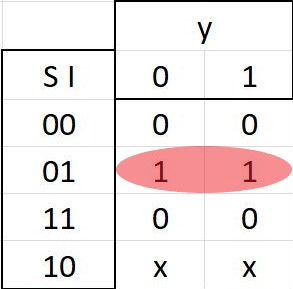
\includegraphics[scale=0.5]{Ej1_Mealy_KY.jpeg}
\par\end{centering}
\caption{Mapa Karnaugh $Y$}
\end{figure}

\[
Y=\bar{S}I
\]

\begin{figure}
\begin{centering}
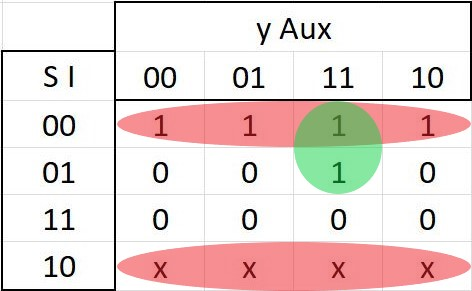
\includegraphics[scale=0.5]{Ej1_Mealy_KB1.jpeg}
\par\end{centering}
\caption{Mapa Karnaugh $B_{1}$}
\end{figure}

\[
B_{1}=\bar{I}+yAux\bar{S}
\]

\begin{figure}
\begin{centering}
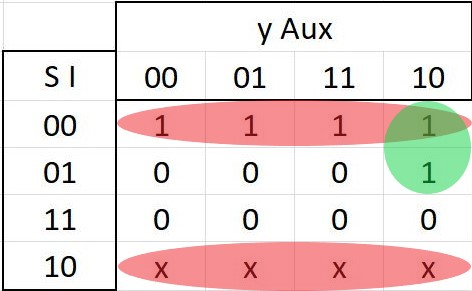
\includegraphics[scale=0.5]{Ej1_Mealy_KB2.jpeg}
\par\end{centering}
\caption{Mapa Karnaugh $B_{2}$}

\end{figure}

\[
B_{2}=\bar{I}+y\bar{Aux}\bar{S}
\]

\end{document}
